\section{Tuesday, April 4th: Native Events -- Widgets, Events, Model-View-Controller}
\subsection{Unexpected Circumstances}
The Professor tested positive for COVID, and thus class will be virtual for today and Thursday.

\subsection{Administrative Matters}
Midterm 1 grades have been released. The midterm was out of 125 points total (though there were up to five extra credit points). The following statistics are about normal for an exam in CS 160.
\begin{center}
    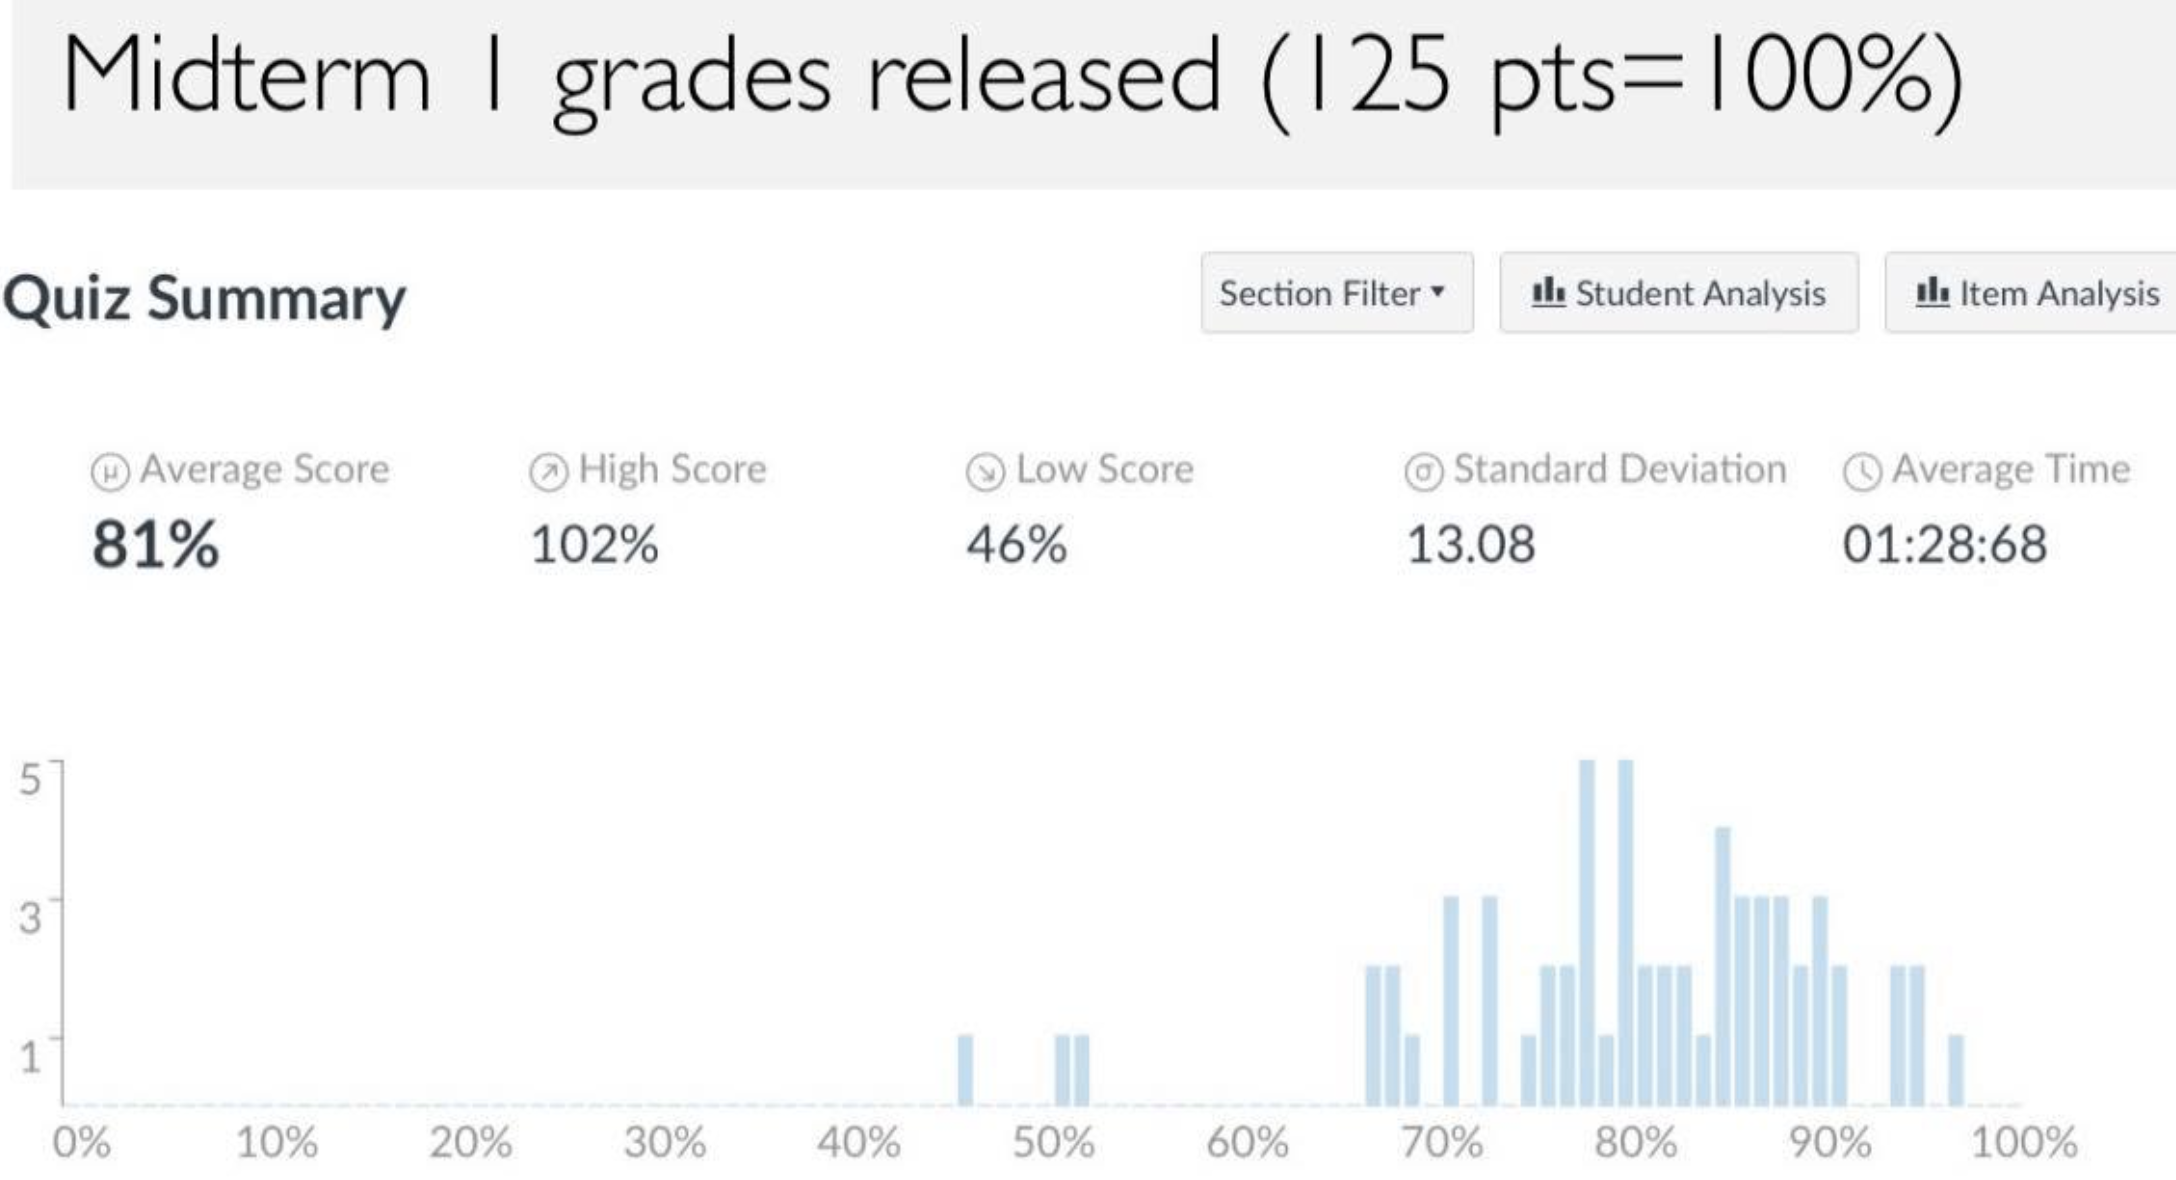
\includegraphics[scale=0.25]
    {lectures/wk11/img/midterm_grades.png}
\end{center}

\subsubsection{Midterm 1 Regrades}
Standard regrade policy applies here to request a regrade, please write a detailed explanation for your request and submitted via the regrade request form that's on the syllabus for the course. Please do that within one week. Do not email directly -- then Course Staff just lose track of all the requests. Make sure to do this especially if the point total on the question does not match the feedback you've been given. Or if we just forgot this to grade something, we're fallible, this happens, sorry, we will fix that. Please do not argue with us about partial credit. Credit on a given question. Since like one person consistently graded a poll question for everyone in the class. And so we tried to be very consistent in how we assign partial credit. So your number is in similar in relation to other students who provided a similar answer. 

\subsubsection{Midterm 2 Logistics}
Midterm \#2 will take place next week, Tuesday April 11th 2023. 

The format will be the same as midterm \#1 -- it will be released the midterm online through bcourses at 09:00 A.M. 

You will have 90 min within a 24-hour time, 24 hour time window to take the exam which will once again have a mix of multiple choice and open answer questions. 
\begin{important}
Midterm \#2 is not cumulative. This is \textbf{not} a final exam. We will only ask about material that was not yet covered in midterm \#1. 
\end{important}

\subsubsection{Scope:}
\begin{shaded}
This means the material we'll cover is that from lectures 14 through 20, information visualization, usability inspection methods, usability evaluation, data analysis, and three lectures on implementation of which we are in the second right now. 
\end{shaded}

\myparagraph{Readings Scope}
Readings: we will not ask you about information visualization readings since we made that optional. We will ask you about the two Martin chapters on experiment design interpreting data. The heuristic evaluation links provided in the heuristic evaluation assignment are also fair game -- they should pretty much match what we covered in class. The last reading on how browsers work is also in-scope.

\myparagraph{Course curving scheme}
Question: Is this class curved?\\
Answer: This class is not usually curved. Usually we get just about what we want in terms of a an upper division or a master's class great distribution by just taking straight values. Usually the exams tend to be a little lower than the project assignments and the homework assignment grades. We will definitely not curved down. We can take a look if all the values are significantly below where they should be. If so, then we curve up but haven't had to do that in the past -- so I would not expect that to happen this year either. 

\subsubsection{Next Team Project Assignment}
The next team project assignment is a heuristic evaluation. Now, heuristic evaluation is a discount usability method as we discussed, that should be quick to do. That's why we only were only assigning one week. And in fact, you will do most of the work for this assignment. In section this week. You will conduct a heuristic evaluation on another team's Figma prototype and vice versa. Another team will evaluate your Figma prototype. This will happen in sections, so it's important to attend section. You will then share the report of what juristic violations you found with the other team within 24 h of section. And you will receive your report and then you as a team, we'll discuss, well, what should we do, what should we redesign based on these usability violations that were found? Briefly write that up, and then submit that to us. So I would say the majority of the work for this assignment happens in section. And then maybe there's another hour or so a team meeting that you should have afterwards to interpret the results. So in the larger scheme of things, this is a much smaller team assignment than the ones you've done previously. If since you submitted your Figma prototypes to us, you've had other ideas, your thinking has evolved. Feel free to iterate and change your Figma prototype. Before this week's section. If you think it's fine, you don't need to do anything. \\
Following this week, we will have three weeks of weekly implementation check-ins in sections. So you will submit a brief progress updates to us. And then in section, meet with your team to work on your project and also check in with your GSI to discuss your progress, what you've accomplished, what remains to be done, what your plan is. So we want you to every week for the following three weeks basically make for here on progress. So you're not keeping it all for a rush at the end. That takes us through the last week of regular classes. During RRR week. We then have our scheduled demo session, that is Wednesday, May 3rd at 02:00 P.M. That's where we will you will show your final demo to class staff and the public. And you will also have a poster about your project. And then during finals week, one week afterwards, we give you one extra week to put together final video and team evaluation. 

\subsection{Native App Concepts}
\begin{itemize}
    \item Native applications provide a “cleaner” and simpler architecture for constructing interactive applications bc that SW stack was built for interactivity
    \item Web apps had interactivity added on top of a document-centric, distributed client-server system
    \item GUI Toolkits
    \begin{itemize}
        \item We don't write the main function
    \end{itemize}

    \item Widgets
    \begin{itemize}
        \item Modular components that get reused again and again
        \item Ex. Android lists or date/time pickers, buttons, toggles, text fields, etc
    \end{itemize}
    
    \item UI Components
    \begin{itemize}
        \item Each component is an object with:
            \begin{itemize}
                \item Bounding box
                \item Paint method for drawing itself
                \item Something else
            \end{itemize}
        \item 2D graphics model
            \begin{itemize}
                \item Typically top left to bottom right
            \end{itemize}
        \item Sizing
        \begin{itemize}
            \item Widgets are not in control, bounding box is controlled by Layout Manager
            \item Component has to know how to draw itself at a size provided by LM
        \end{itemize}
    \end{itemize}
    
    \item Working with Widgets
    \begin{itemize}
        \item Make common case fast, uncommon case possible
        \item Common case: assemble standard widgets into a layout
        \begin{itemize}
            \item Instantiate class, provide configuration parameters
        \end{itemize}
    
        \item Uncommon case: write your own widget
    \end{itemize}
    
    \item Absolute layout
    \begin{itemize}
        \item Good idea? Provide absolute coordinates for everything
        \begin{itemize}
            \item Bad idea in general outside of prototyping, hardcoding parameters only works for a given screen size
        \end{itemize}
    \end{itemize}
    
    \item Event Dispatch Loop
    \begin{itemize}
        \item Mouse moved = Event Queue (sorted queue of input events) → Event Loop (runs in dedicated thread)
        \begin{itemize}
            \item Event Loop:
            \begin{itemize}
                \item Remove next event from queue
                \item Determine event type
                \item Find proper components
                \item Invoke callbacks on components
                \item Repeat or wait until event arrives
            \end{itemize}
        \end{itemize}
        
        \item $\to$ Component (invoked callback method, update application state, request repaint if needed)
    
        \item Model-View-Controller
        \begin{itemize}
            \item Model
            \item View
            \item Controller
            \begin{itemize}
                \item Receives input events from user, decides what to do by talking to view to determine which objects are being manipulated
                \item Calls model methods to make changes on objects
                \item Model then notifies views to change
            \end{itemize}
        \end{itemize}
    
        \item Why MVC?
        \begin{itemize}
            \item Combining MVC into one class will not scale
        \end{itemize}
    \end{itemize}
\end{itemize}
